\documentclass[a4paper]{article}
\usepackage[utf8]{inputenc}
\usepackage[english]{babel}
\usepackage{url}
\usepackage{graphicx}
\usepackage{array}
\usepackage{geometry}
\usepackage{tabularx}
\usepackage{pgfplots}
\usepackage{amsmath}
\usepackage{amsfonts}
\usepackage{amssymb}
\usepackage{placeins}

\setlength\parindent{0pt}

\title{Intelligent Patient Record}

\author{ITU \\
\vspace{5mm}
Mathias Schmidt, Thomas Snaidero \\
Supervisors: \\
Steven Houben, Mads Frost}

\date{21 May 2014}

\begin{document}

\maketitle
\pagebreak
\tableofcontents
\pagebreak


\section{Introduction}


We have had the task of build a new revision, of Steven Houben Hyper Record.

One of the big reasons is it was to unwieldy and heavy for the medical staff.


\section{Design requirements}

Houben et al.'s proposed device shown on figure \ref{fig:old-hypr} was taken as a reference, with regards to weight, thickness and size. Although the new design retains the same purpose, the feature of having a dock for a tablet was removed, to further reduce the size. The hybrid patient record was then re-imagined to be just a thin support for a folder, with electronics on the back. \\

Working from Houben et al.'s proposed device, a new set of requirements have been established, in order to improve on the design. The following is a list of requirements pertaining to the new device:

\begin{itemize} \itemsep0em
	\item Weight: less than 500g
	\item Thickness: less than 20mm
	\item Size: Approximately same dimensions as A4 paper
	\item Maintainability: easy access to the microcontroller's programming interface
	\item Maintainability: easily change components without changing physical design
\end{itemize}

A set of requirements pertaining to the electronic part of the device has also been decided:

\begin{itemize} \itemsep0em
	\item Rechargeable battery via standard USB cable
	\item Battery status LEDs
	\item Autonomy of at least 8 hours on battery, with normal use
	\item LEDs showing colour combinations should be easily seen and understood from 10m 
	\item Hear the audio signal in a room, when device is under bed sheets
\end{itemize}

\begin{figure}[h]
\begin{center}
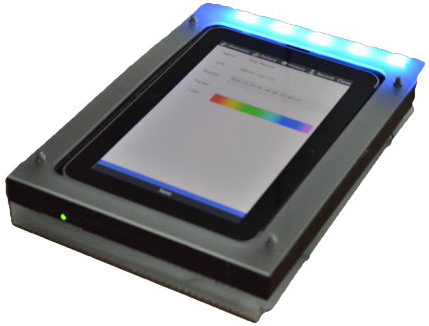
\includegraphics[scale=.5]{figures/old-hypr.jpg}
\caption{\small {\it {This is a description}}} \label{fig:old-hypr}
\end{center}
\end{figure}
% Numbered list of product requirements with most important first, least important last.

%\section{Use case scenarios}
% Detailed description of 3 use case scenarios which illustrate:
% - The user experience
% - Insight about a specific product feature, or user requirement

%\section{Design analysis and concept diagrams}
Description of issues related to the design of the product:
- Description of concepts, requirements and features of the product
- Review of motivations for making the design decisions
- Indicate the primary features of the design that are the most creative and original

\subsection{Materials}
We got a bunch of different plast materials from RIAS, in order to find some material that might be cheaper, and better that acrylic, since acrylic have tendency to be brittle, this becomes worse when it has been laser cut. 
PEHD
RIALEN PP
PETG
PP-H
ACRYL
POM-C

PEEK
PPSU

\subsection{Iterations}
we have used prototyping in order to get a viable device, through the different designs we have been able to see different problems, which have ment that we had to iterate to a new version, we have been limited by time, so we have had to make some compromises

\subsubsection{fisrt}
The first iteration that we build did have some problems.
The first is that it is expensive to build, since we are using a lot of acrylic, the secound point is that it still is heavy, and unwieldy.
But i did give some ideas for the next iteration.

\subsubsection{secound}


\subsubsection{thried}


\subsubsection{fourth}


\subsubsection{fith}

\subsubsection{sixth}


% Description of issues related to the design of the product:
% - Description of concepts, requirements and features of the product
% - Review of motivations for making the design decisions
% - Indicate the primary features of the design that are the most creative and original

\section{Materials}

- materials description
- 

\section{Theory}
\subsection{Rapid prototyping}

% Sources: \\
% (1) $books.google.com/books?id=4OYcyiDUpsQC$ \\
% \cite{efunda} $efunda.com/processes/rapid_prototyping/intro.cfm$ \\
% (3) $http://en.wikipedia.org/wiki/Fused_deposition_modeling$ \\
% \cite{slic3r} $http://slic3r.org/$
% \cite{wiki3D} $http://en.wikipedia.org/wiki/3D_Printing$ \\

Prototyping of a physical product is an age old process that has evolved all the way to today. Up until the emergence of virtual prototyping with CAD applications, prototyping was manual, and tended to be craft-based, thus very slow \cite{chua2010}. \\
In the 1980s, virtual prototyping became more widespread, as computer tools became more mature. Virtual models could now be analysed and modified as if they were physical prototypes, and several iterations of designs could be easily carried out. But as the prototypes became more complex, the time required to make a physical model increased, and therefore craft-based production of a physical prototype became tedious \cite{chua2010}. \\

A new type of prototyping has therefore emerged in the 1980s, called rapid prototyping (RP). Rapid Prototyping can be defined as techniques used to quickly fabricate a scale model of a part or assembly, using three-dimensional computer aided design (CAD). \\

Rapid Prototyping has also been referred to as solid free-form manufacturing, computer automated manufacturing, and layered manufacturing \cite{efunda}. An RP model's most used scenario is for testing various qualities of a physical product, and in some cases, the RP part can be the final part, but typically the RP material is not strong or accurate enough. \\

There exists many experimental RP techniques such as Stereolithography (SLA), Digital Light Processing (DLP), Laminated Object Manufacturing (LOM), Electron Beam Freeform Fabrication (EBF3), Fused Deposition Modelling (FDM), and more \cite{wiki3D}. The latter was specifically used in this project, because of its almost ubiquitous presence in universities, fab-labs, and hackerspaces. \\

The main reasons for using Rapid Prototyping are very compelling. It decreases costly mistakes and engineering changes, thus minimizing development time. By being able to have a look at the product early in the design process, mistakes can be corrected, and changes can be made while they are still inexpensive. \\

Rapid prototyping can be performed in many different ways, but they all adopt the same basic methodology:

\begin{itemize} \itemsep0em
  \item A virtual model is designed in a CAD application.  It represents the part that is physically built as an enclosed volume, and will specify the inside, the outside, and boundaries of the model.
  \item The model to be built is next converted into an STL (Stereo Lithography) file format. The STL format approximates the surfaces of the model by polygons.
  \item A program analyses the STL file, and ``slices'' the model into cross-sections. It generates paths to be filled and calculates the amount of material to be extruded, in the case of a 3D printer that uses fused deposition modelling \cite{slic3r}. In short, it converts a digital 3D model into printing instructions for a 3D printer.
  \item The model and any supports are removed. The surface of the model is then finished and cleaned for imperfections \cite{efunda}.
\end{itemize}


\section{Methods}
\subsection{Software}
For the Design we have used openscad, and steard away from 3d design programs like 3d studio max and blender.
The reason is when you design a file in 3d studio max or blender, it might look big, and you may have followede the messurments in the program, you usual have to multiply the figur by a factor of 1000x due to conversion problems. Beside that you can have problems with the node points in the design, some times the design file might lock like all the points that need to be conected are, but when you multiply the figure by a factor or zoom up close, that might not be true, and that can give problems.
The othere is the avalibity and price, openscad is a simple, lightwitght and opensource program that is easy to learn and use for programmers, since you create objects if by writing simple code ex. Cube([5,5,5]); 
We could have bought a linces for some other program like autocad or different cad program, but we found the unessery since it is simple 3D models, and we don't need a huge program for that.

When the design is done we have exportede the openscad file to STL, that we have but into scli3r, that are one of the best stl to gcode convert there exsist, where you take stl files that are exportede from openscad and convert them to gcode, which is instruction code that the firmware on the 3D printer understand. beside that it is openscource, and is used for almost all 3d printeres.

For the laser cutting we have used inkscabe, which also is an opensource program, the reason is that we only had to change the line thickness on the DXF file that was exported from openscad. and save it as an pdf. 

\subsection{Machines}
\subsubsection{3D Printers}
There is a lot of different 3D printers design, the printers that we had access to was prusa i3 at ITU, and MAXbot in labitat, they work in the same way, with it's x,y  and z axsis, the main differense is the thickness of the pla that they use, geearing and how the bed is cunstructed. The prusa i3 at ITU usses 3mm pla vs MAXbot that uses 1.75 mm pla, this has the complecation that prusa need to have a gearing system in order to give enough pressur.
The last main difference is that the Prusa i3 don't have any springs in the bed, which can leed to some problems where the nossel get attach ot the print and force it of the plate.

\subsubsection{Laser cutter}
For the laser cutting we have used the 60W laser at ITU, we did have some back up at some different fablabs, if the laser stop working.

\section{Iterations}

The following four prototype iterations shown on figure \ref{fig:v1} to \ref{fig:v5}, depict an exploded view of the design on the left, and the physical version on the right. There is one major change in design during the process from prototype two to three, but they have all one thing in common: the journal is meant to be fixed on top of an acrylic sheet. \\
The first two prototype ideas shown on figures \ref{fig:v1} and \ref{fig:v2} were made entirely with acrylic sheets cut with a laser-cutter, and the two remaining ones, a mix of laser cutting, and 3D printing.

\subsection{First iteration}
The first prototype on figure \ref{fig:v1} was designed to accommodate eight banks of 4 x 1,5V AAA batteries. Compartments for each electronic component were made to place them on a flat surface, and reduce thickness. A box on the left of the journal was meant to hold LEDs. This design had many flaws however -- the list below describes the various issues.

\begin{itemize} \itemsep0em
  \item It felt heavy, and the weight exceeded 500g.
  \item The sharp edges from the laser-cut acrylic were slightly uncomfortable.
  \item The sheets were glued together, and made the case impossible to open.
  \item The glueing process is tedious because of the tools needed, and the hardening takes 24h.
  % \item Compartments were engraved with the laser-cutter, which requires constant supervision of the cutting.
  \item Problems with displacement of compartments from the different acrylic sheets.
  \item No charging possibility.
  \item Wiring of components was difficult.
  \item The side piece made it difficult to open the journal.
\end{itemize}

A few positive characteristics were observed:
\begin{itemize} \itemsep0em
  \item Removal of protruding bolts.
  \item Reduced thickness by 15mm.
\end{itemize}


\begin{figure}[h]
\begin{minipage}[b]{.5\textwidth}
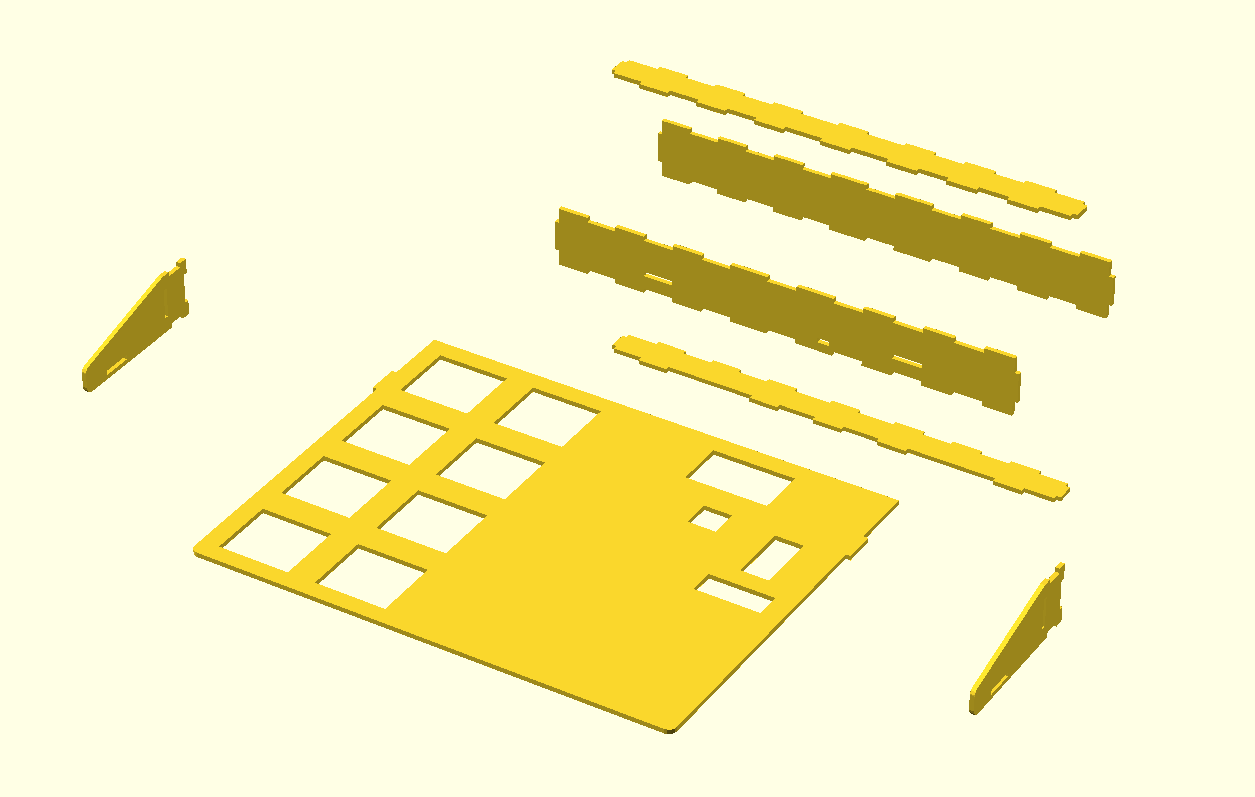
\includegraphics[width=1.05\textwidth]{figures/iterations/v1.png}
\end{minipage}
\begin{minipage}[b]{.5\textwidth}
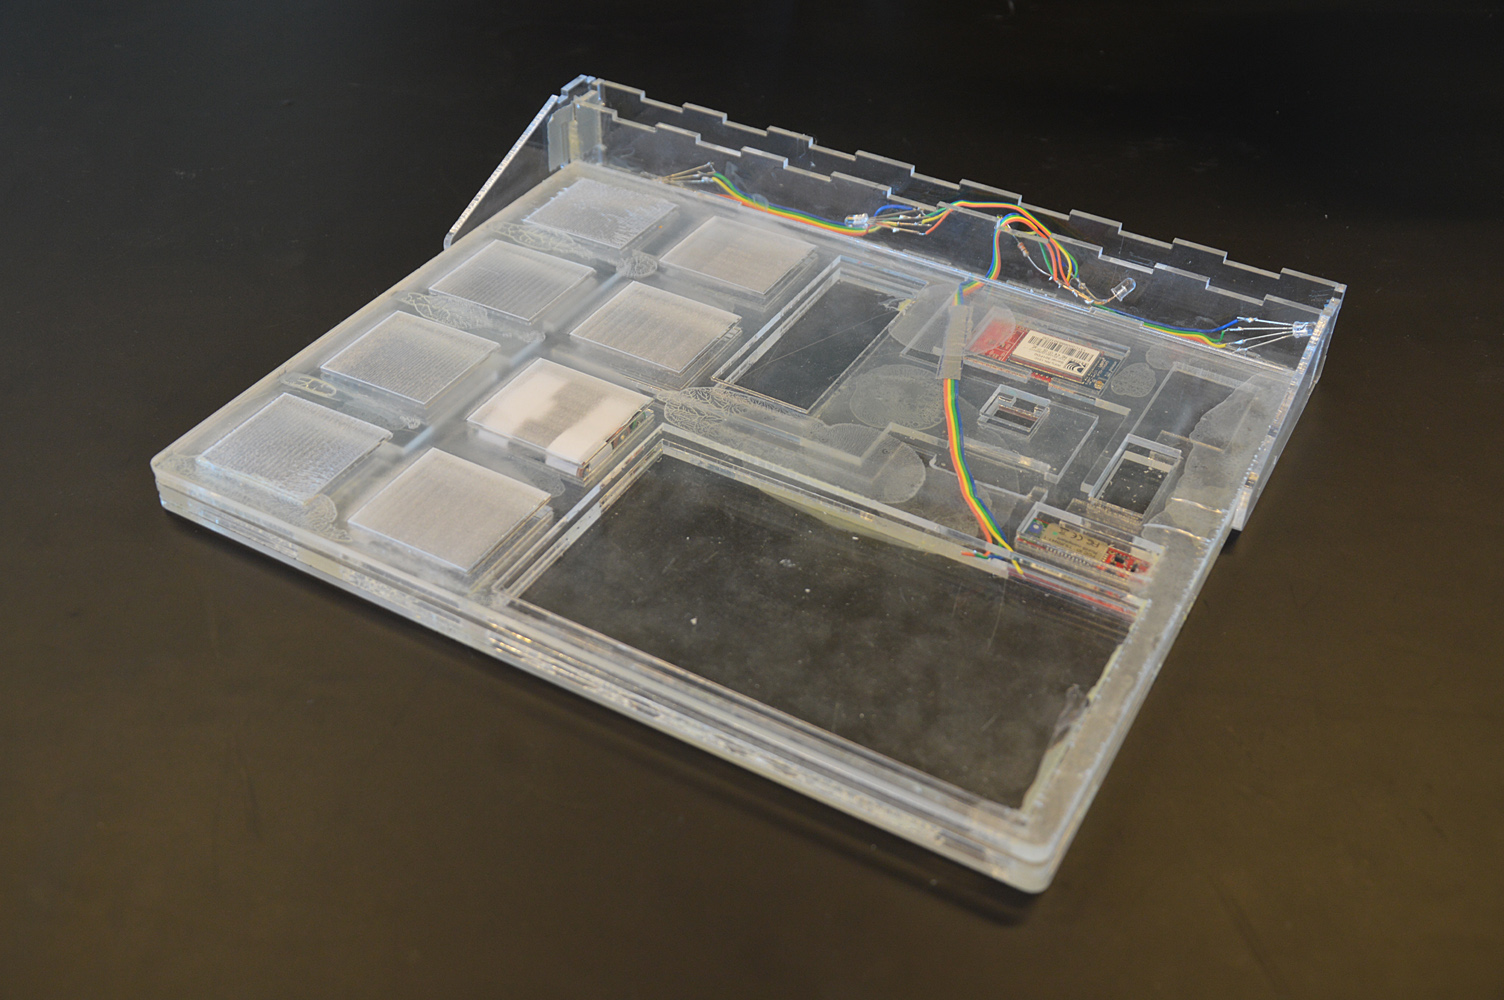
\includegraphics[width=1\textwidth]{figures/iterations/v1-photo.jpg}
\end{minipage}
\caption{\small {\it {The first prototype idea}}} 
\label{fig:v1}
\end{figure}

% -------------------

\subsection{Second iteration}
The second prototype took the previous downsides into consideration, and produced the device shown on figure \ref{fig:v2}. The idea here, is that the electronics were to be moved to a box at the bottom of the journal, in order to make the journal feel less bulky while holding it.

\begin{figure}[h]
\begin{minipage}[b]{.5\textwidth}
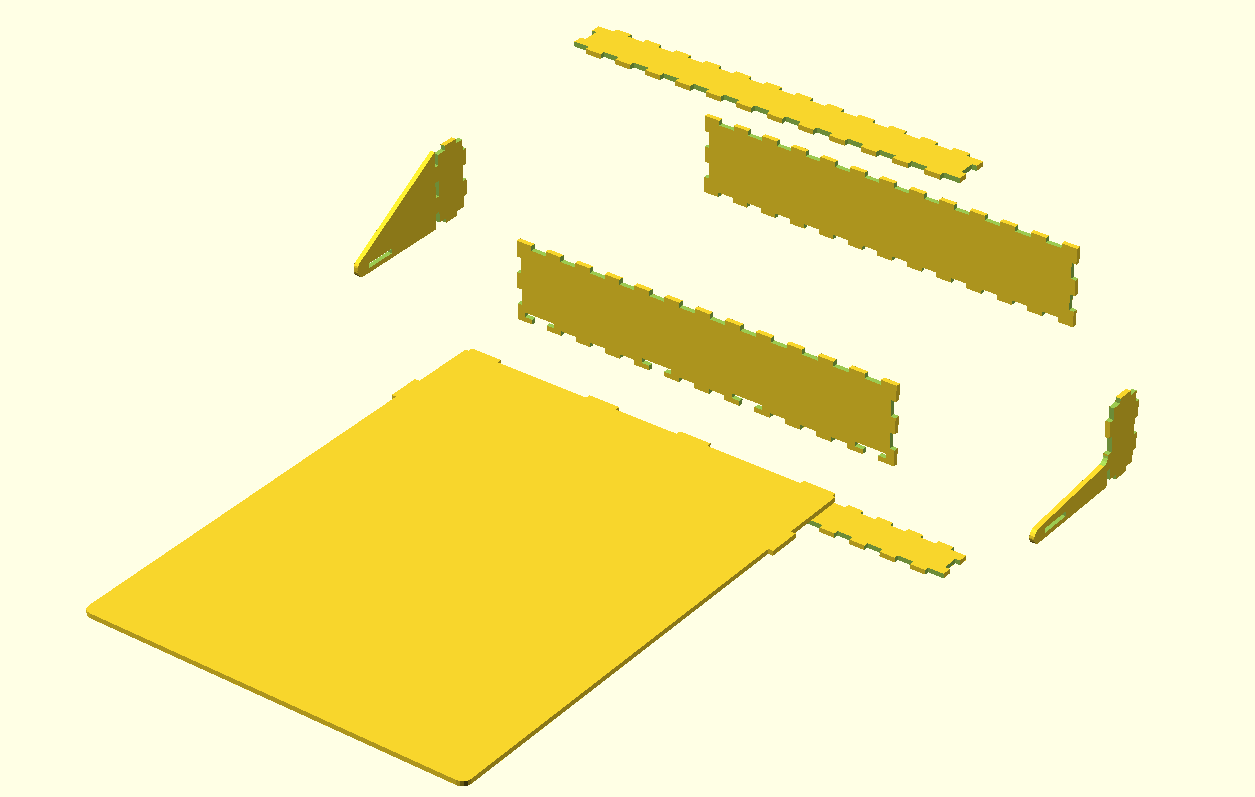
\includegraphics[width=1.05\textwidth]{figures/iterations/v3.png}
\end{minipage}
\begin{minipage}[b]{.5\textwidth}
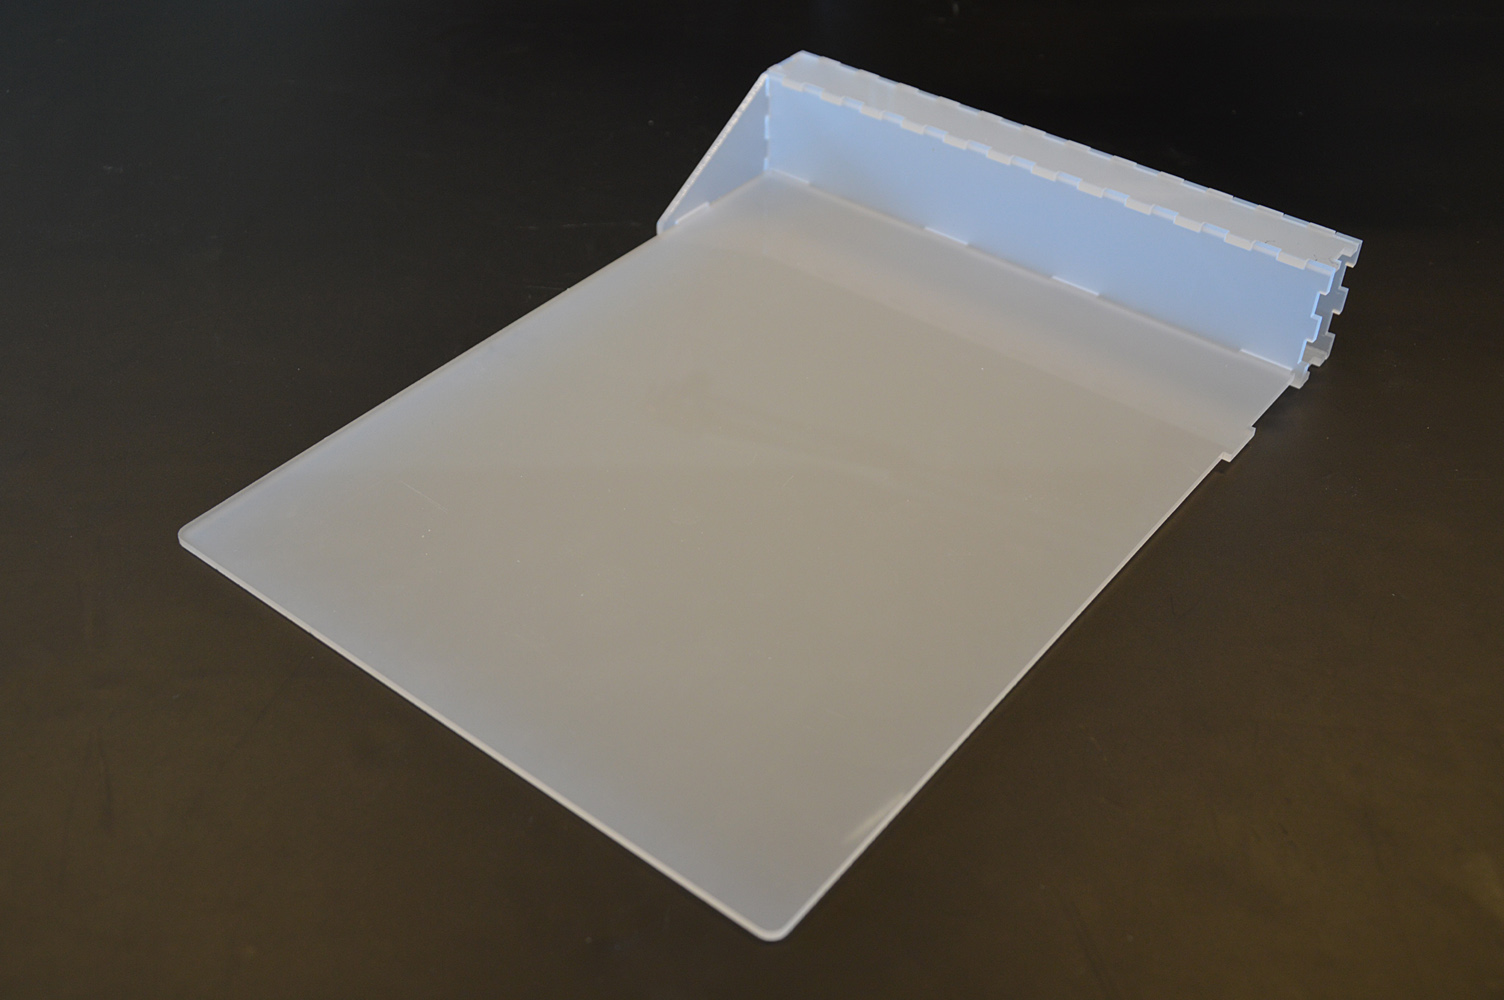
\includegraphics[width=1\textwidth]{figures/iterations/v3-photo.jpg}
\end{minipage}
\caption{\small {\it {The second prototype idea}}} 
\label{fig:v2}
\end{figure}

Following are the issues found with this design.

\begin{itemize} \itemsep0em
	\item Not very pleasant to hold, as the box holding the electronics ended up getting in the way of the user.
	\item Impossibility of performing maintenance, due to the acrylic being glued.
	\item Structurally unsound design - attachment of box to the sheet was flimsy, and broke easily.
	\item No charging possibility.
	\item The weight distribution would have been very uneven, due to the placement of box at the bottom.
\end{itemize}

This prototype was discarded before an attempt to place the electronics in the box, due to the obvious disadvantages. The technique of laser-cutting acrylic sheets and using glue to attach them together proved to be a slow and tedious task. Due to the difficulty of using screws to assemble the parts and using glue instead, made the designs unmaintainable. Complex laser-cut acrylic parts also tended to become brittle, so a rethinking of the design was in order. Using acrylic wasn't out of the question, but the complexity of those parts had to be reduced, and the use of 3D printed PLA for those parts were later introduced. \\

% -------------------

\subsection{Third iteration}

Figure \ref{fig:v3} depicts the third prototype. The electronics were moved to a new 3D printed container made of PLA. The latter was further divided into smaller compartments made for housing the various electronic components. The container had a lid that was screwed on top. \\
The box was also designed to be slid into a sheet of acrylic. Two small protruding triangles where cut in the acrylic sheets in order for them to bend, and the box would then ``click'' into place. The purpose of such system is to make maintainability easier - one would simply have to slide the box out, perform a software update and slide it back in. This was however difficult to get right, and the bending acrylic ended up breaking quickly. Figure \ref{fig:v3} shows the broken acrylic on the right. Two holes on the side were also added to hold an RGB LED, and the other to hold the USB charger intake.

\begin{figure}[h]
\begin{minipage}[b]{.5\textwidth}
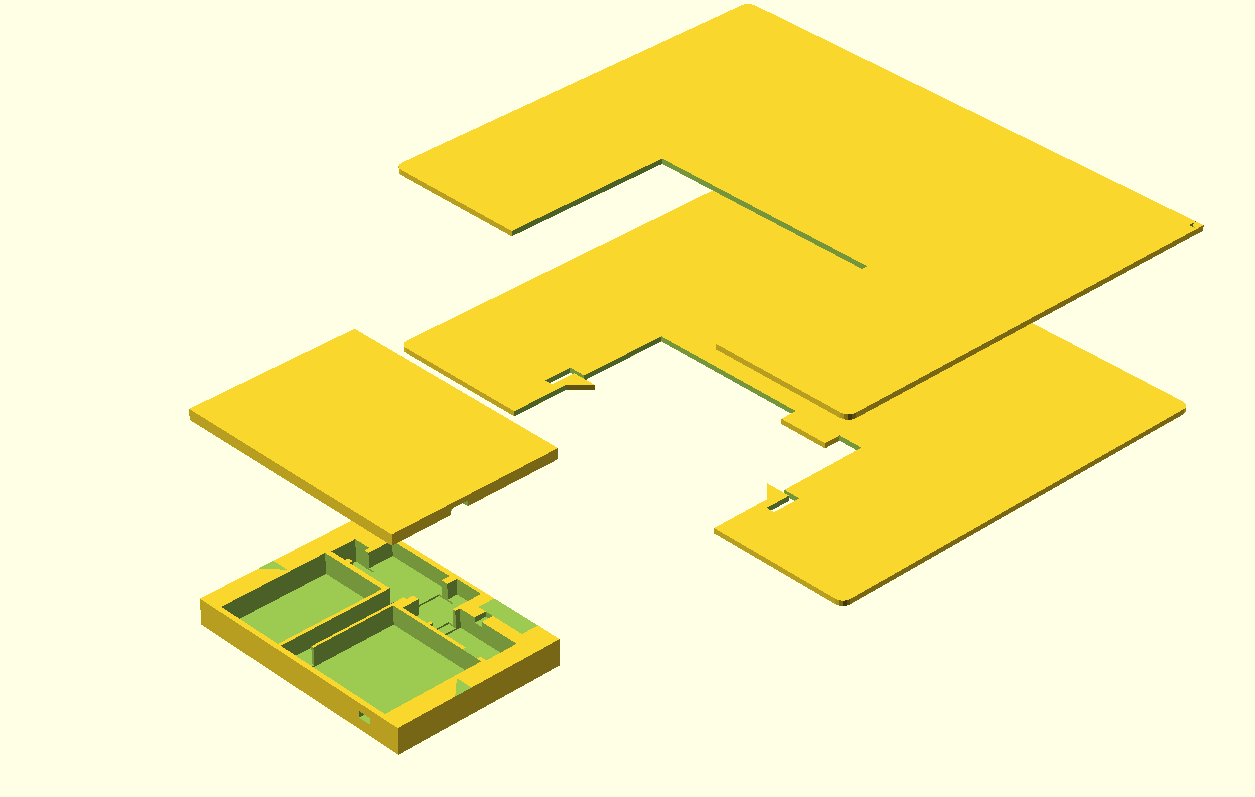
\includegraphics[width=1.05\textwidth]{figures/iterations/v4.png}
\end{minipage}
\begin{minipage}[b]{.5\textwidth}
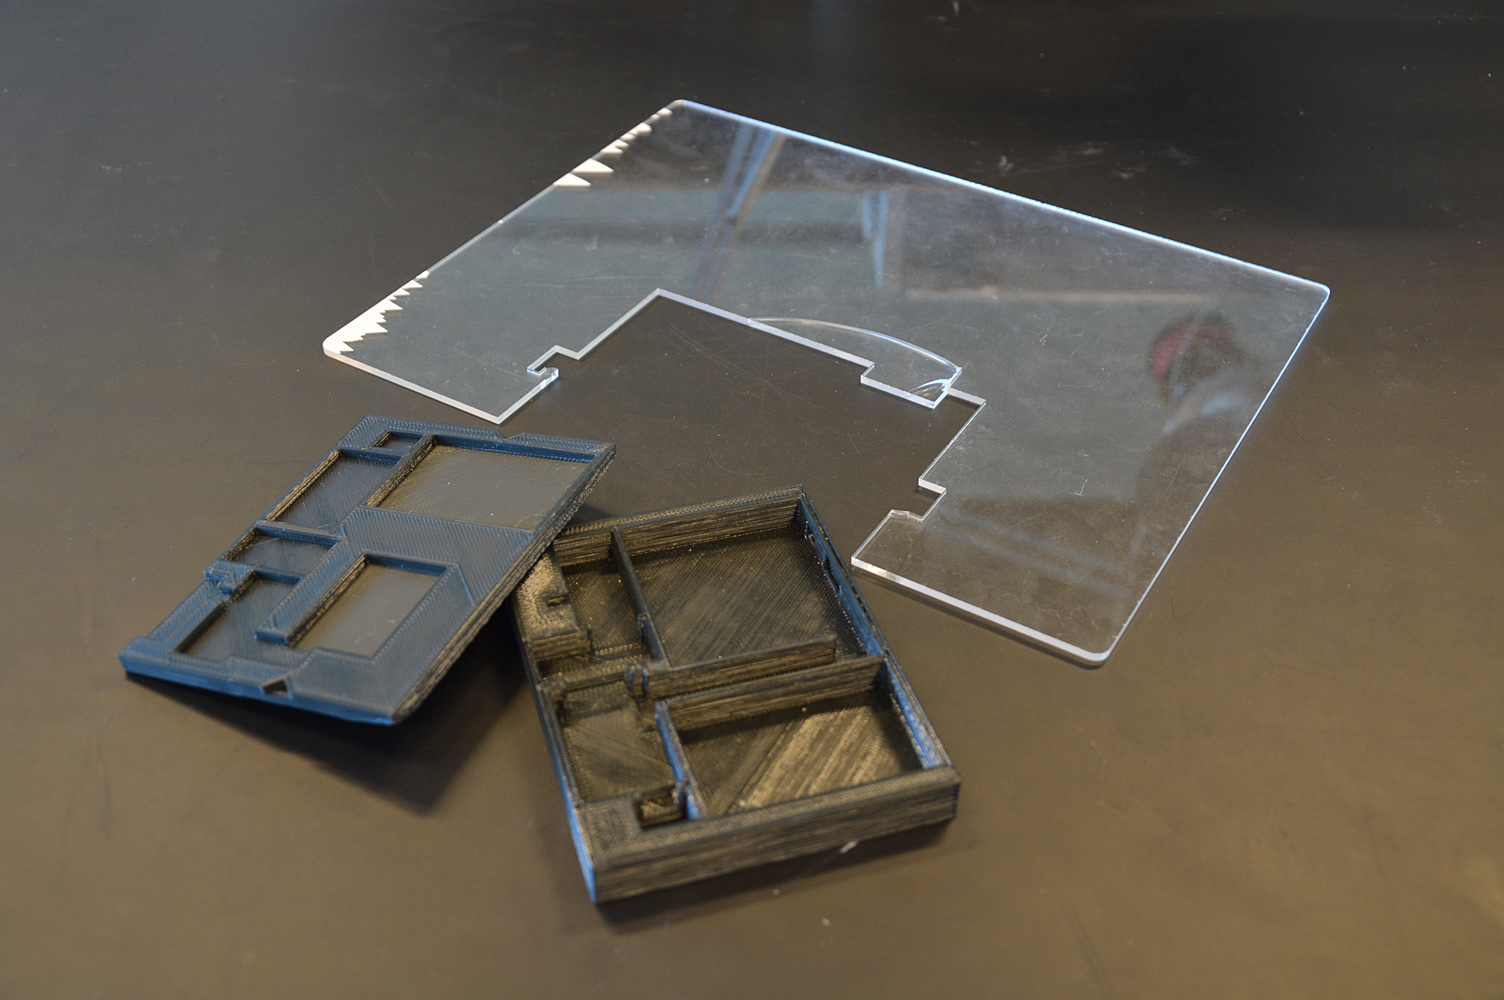
\includegraphics[width=1\textwidth]{figures/iterations/v4-photo.jpg}
\end{minipage}
\caption{\small {\it {The third prototype idea}}} 
\label{fig:v3}
\end{figure}

Following are the issues found with this design:

\begin{itemize} \itemsep0em
  \item The compartments for the electronic components ended up making the wiring of the latter unnecessary complex.
  \item The click system was difficult to achieve with acrylic.
  \item The chosen RGB LED's colours were difficult to discern.
\end{itemize}

This prototype attempted however to resolve many problems found in the previous iterations, and the following positive attributes were observed:

\begin{itemize} \itemsep0em
  \item Comfortable to hold.
  \item Maintenance is easier to perform.
  \item Battery charging via standard mini-USB cable.
  \item The electronics were moved out of the way of the user.
  \item Better weight distribution when holding the journal.
  \item 3D printing opened up possibilities to radically change the design.
\end{itemize}

% -------------------

% \begin{figure}[h]
% \begin{minipage}[b]{7.5cm}
% \centering
% 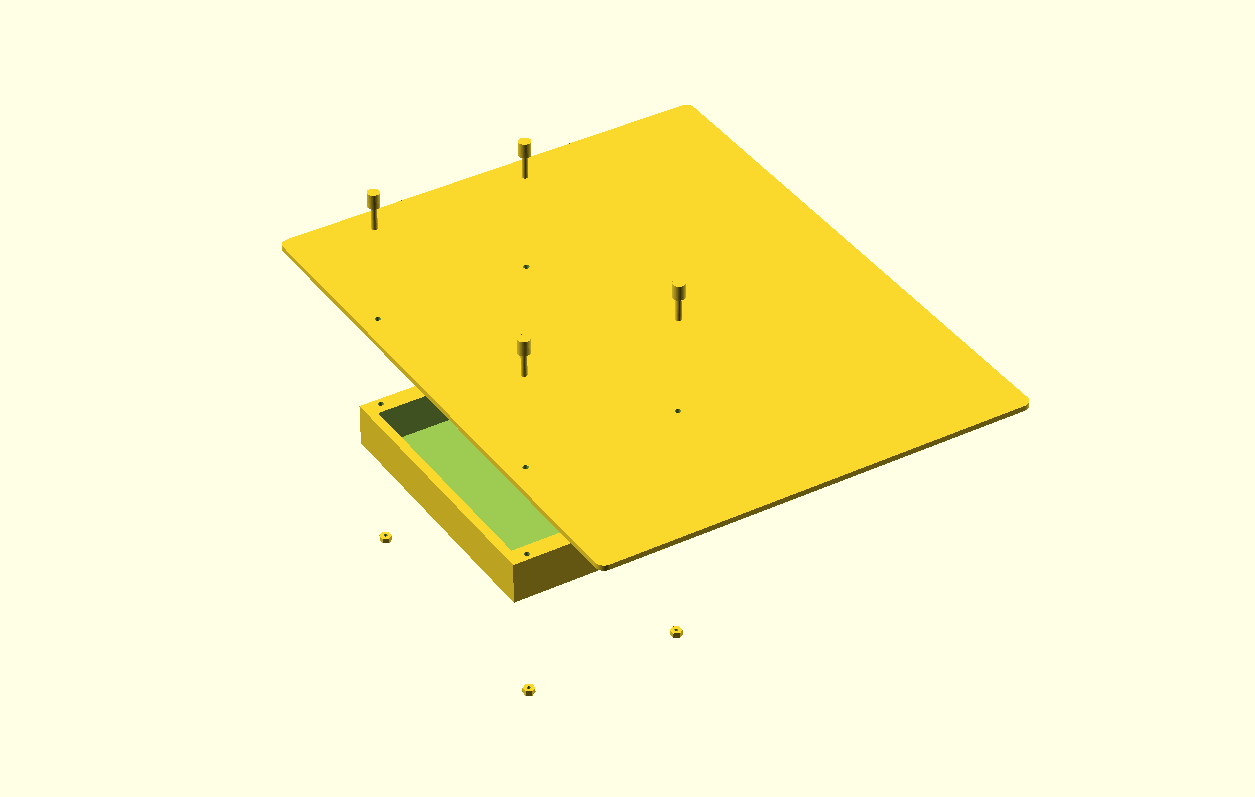
\includegraphics[scale=0.235]{figures/iterations/v5.png}
% \end{minipage}
% % \hspace{0.5cm}
% \begin{minipage}[b]{7.5cm}
% \centering
% 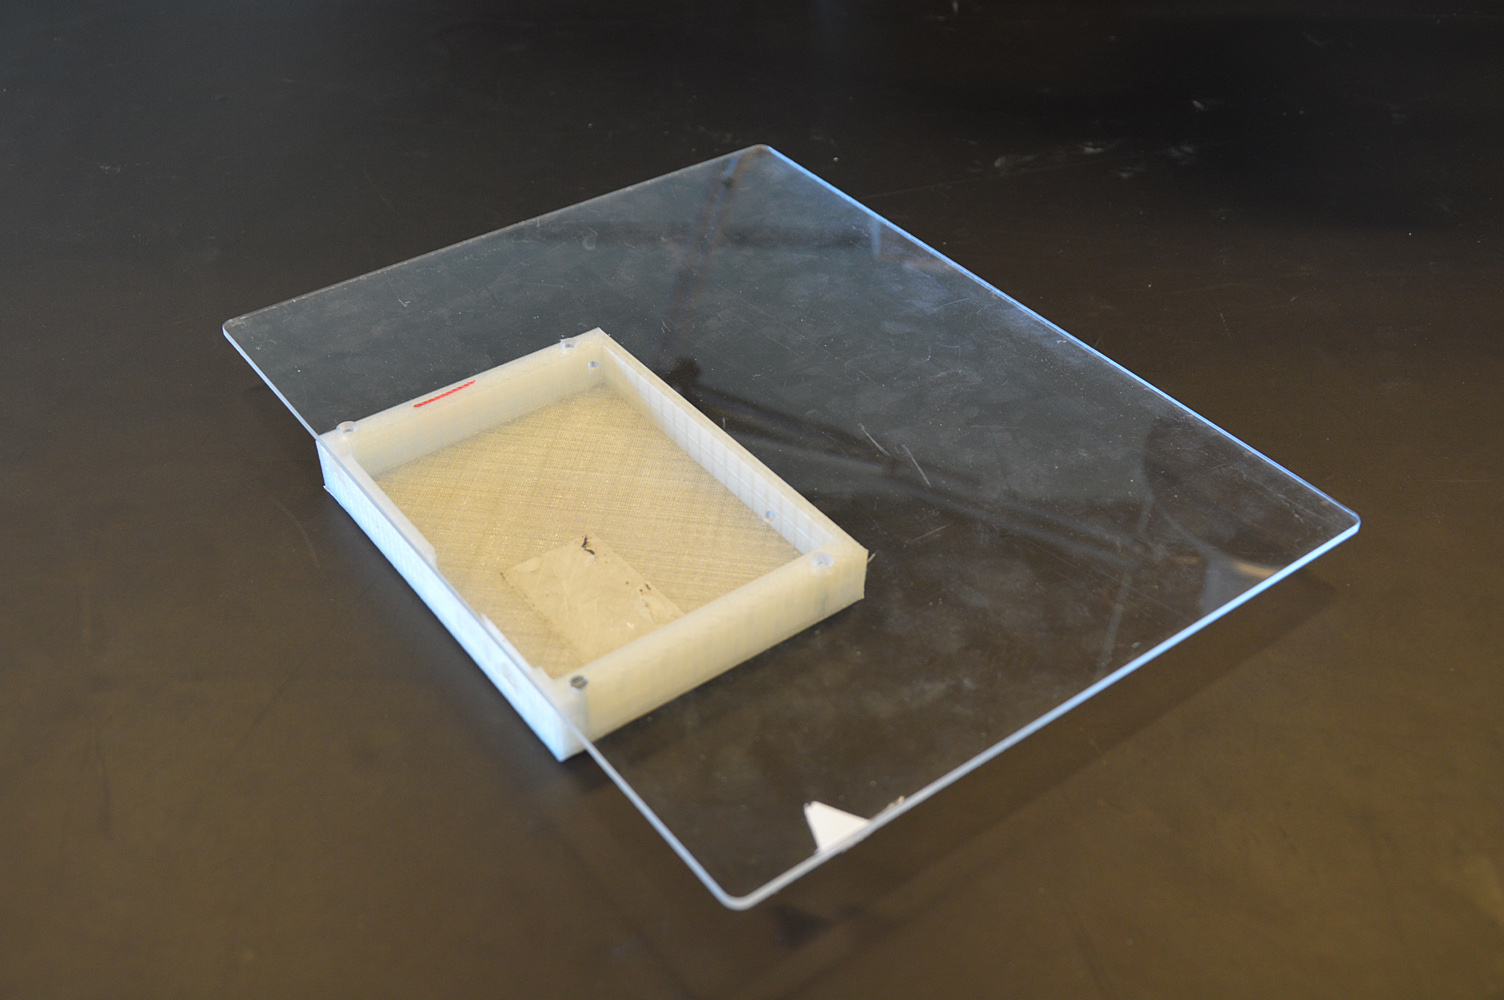
\includegraphics[scale=0.58]{figures/iterations/v5-photo.jpg}
% \end{minipage}
% \caption{\small {\it {The fourth prototype idea}}} \label{fig:v4}
% \end{figure}

% -------------------

\subsection{Fourth iteration}

The fourth prototype shown on figure \ref{fig:v5} was the last iteration made within the available time constraint. The electronics compartments were removed, in favour of one single room for the Arduino, Wifi module, RFID reader, and the battery, and another room for the ultrasonic tracker. The electronics were now wired on a breadboard, which made the system thinner, and easier to maintain as opposed to single elements wired together. The slide system was also improved, and required no bending acrylic parts - a rail was added to the 3D printed lid, where the acrylic sheet is supposed to slide in. The screws were then tightened, which resulted in tightening the box to the acrylic sheets, thus making it hold on to it. This ensured a way to easily slide the box out, when in need for maintenance. A small hole was added at the bottom, to access the battery charger's battery state button. The PLA chosen for the 3D printing was in this case semi transparent, which allowed to place LEDs behind the material, and see the colours distinctly.

\begin{figure}[h]
\begin{minipage}[b]{.5\textwidth}
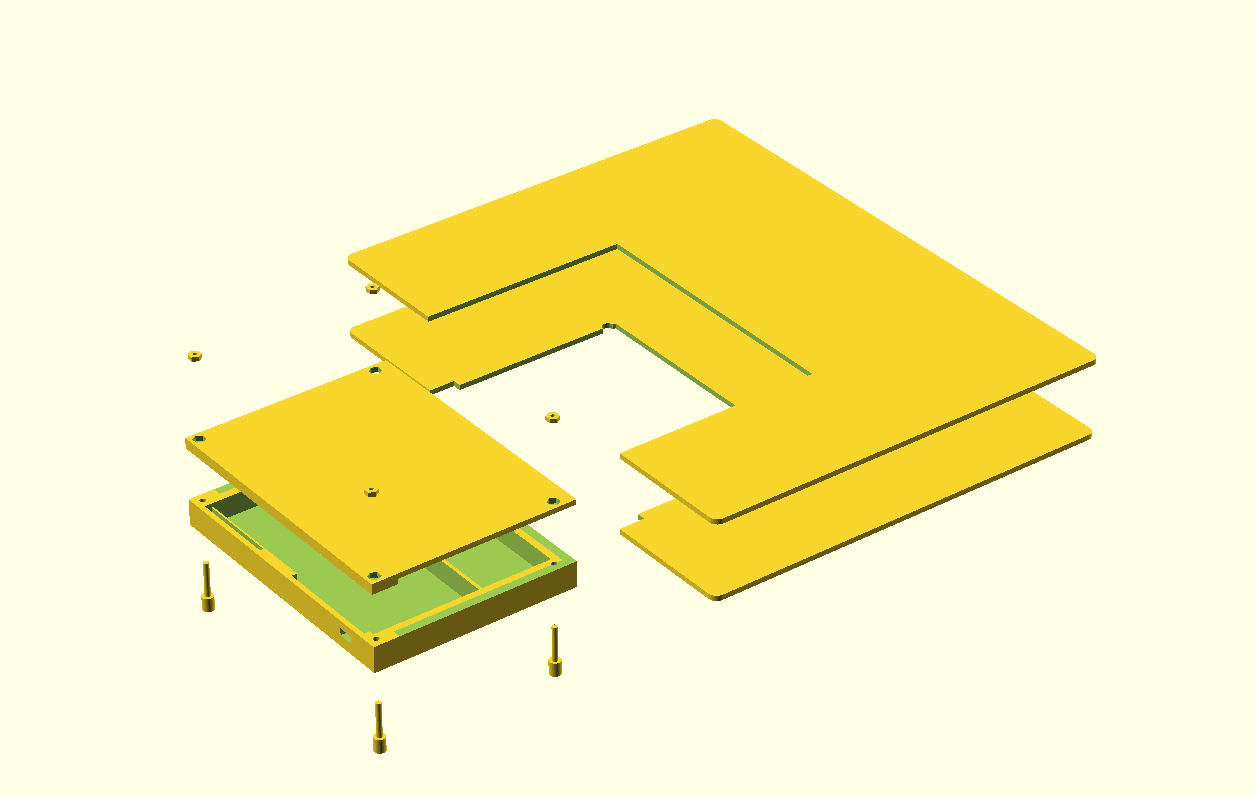
\includegraphics[width=1.05\textwidth]{figures/iterations/v6.png}
\end{minipage}
\begin{minipage}[b]{.5\textwidth}
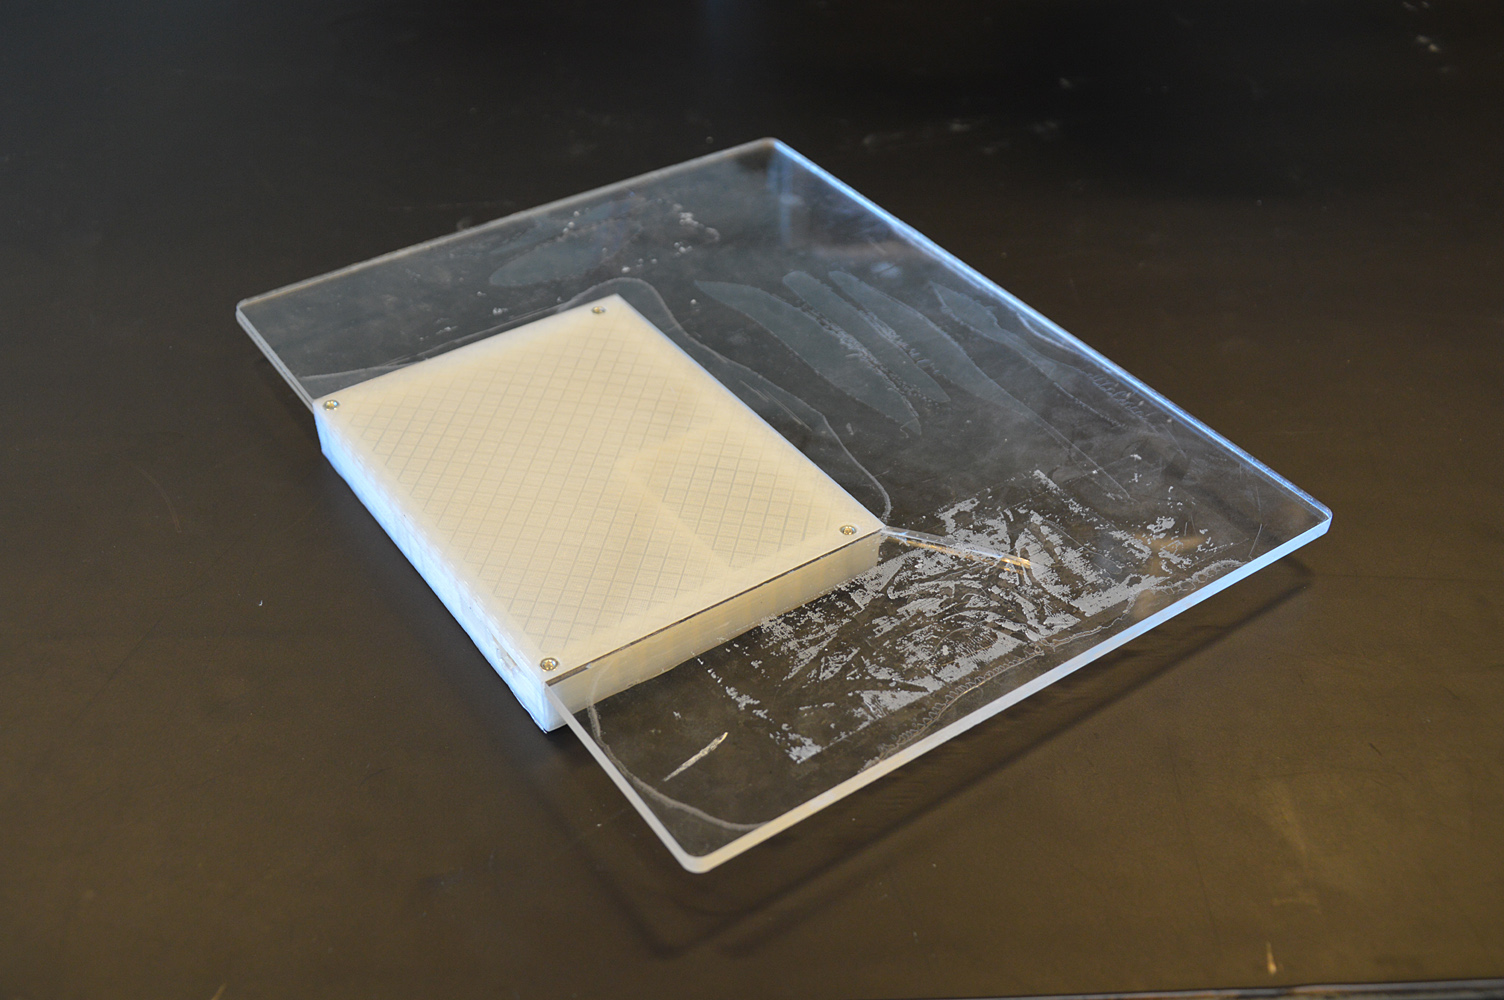
\includegraphics[width=1\textwidth]{figures/iterations/v6-photo.jpg}
\end{minipage}
\caption{\small {\it {The fourth prototype idea}}} 
\label{fig:v5}
\end{figure}

The previous disadvantages were assessed, resulting in the following additional positive observations:

\begin{itemize} \itemsep0em
  \item The electronics were finally able to fit in the box without any hassle.
  \item The slide system worked as intended.
  \item The chosen RGB LED's colours were easily discerned.
\end{itemize}

% -------------------------------------------------------------------------------

\begin{figure}[h]
  \makebox[\textwidth][c]{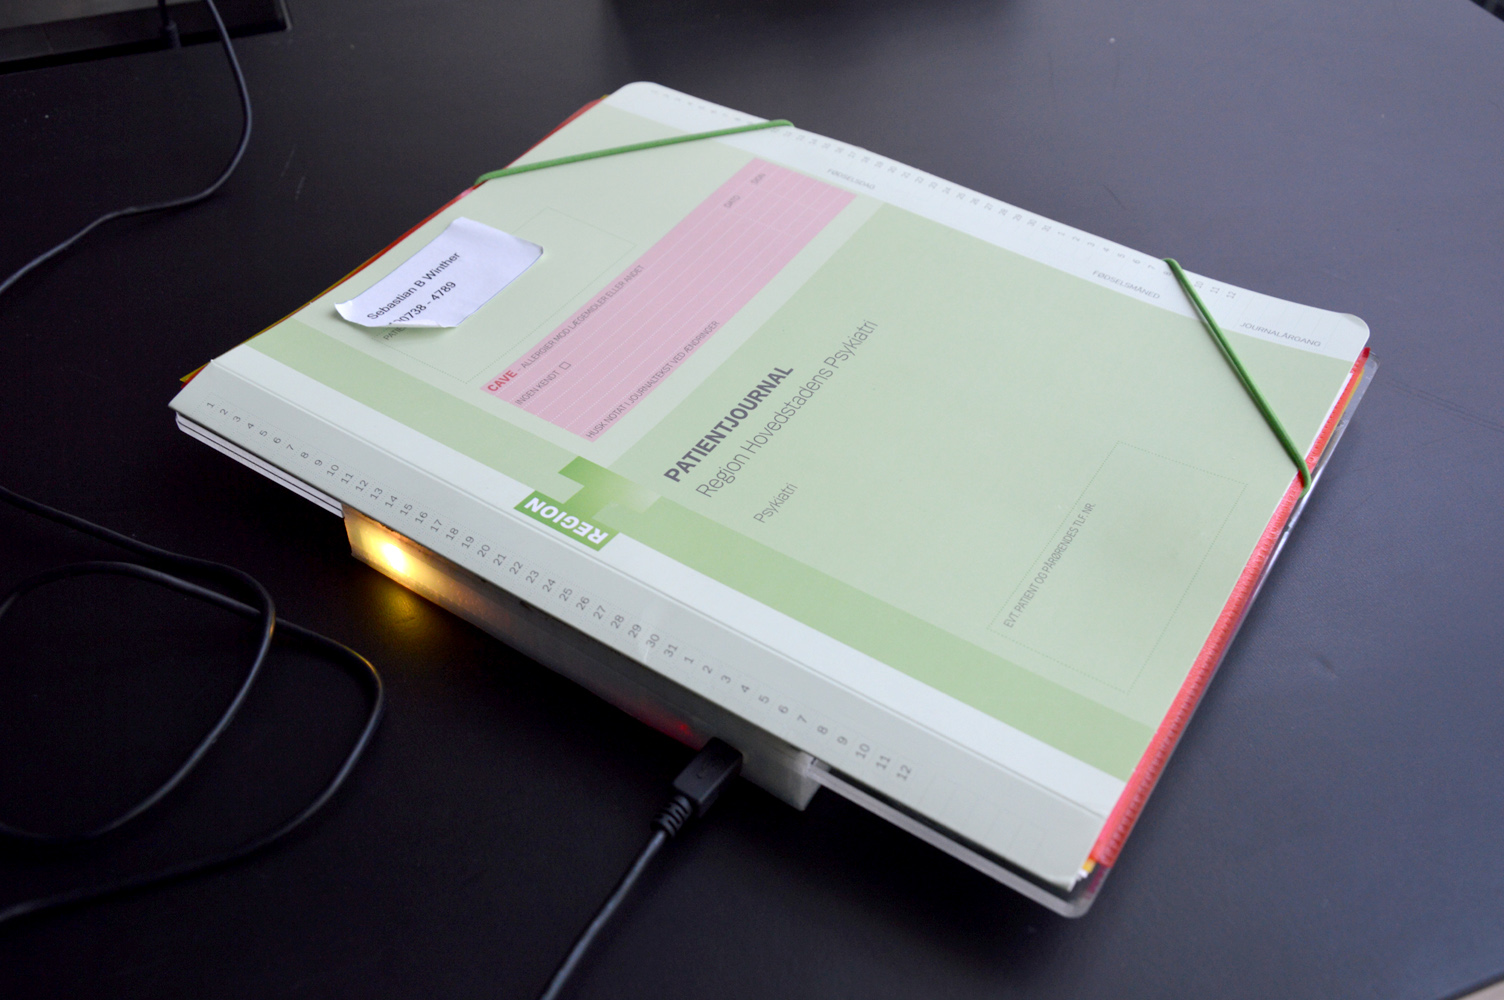
\includegraphics[width=1\textwidth]{figures/journal-1.jpg}}
  \caption{\small {\it {The finished Hybrid Patient Record with a paper journal and connected to a charger.}}} 
  \label{fig:journal-1}
\end{figure}

\begin{figure}[h]
  \makebox[\textwidth][c]{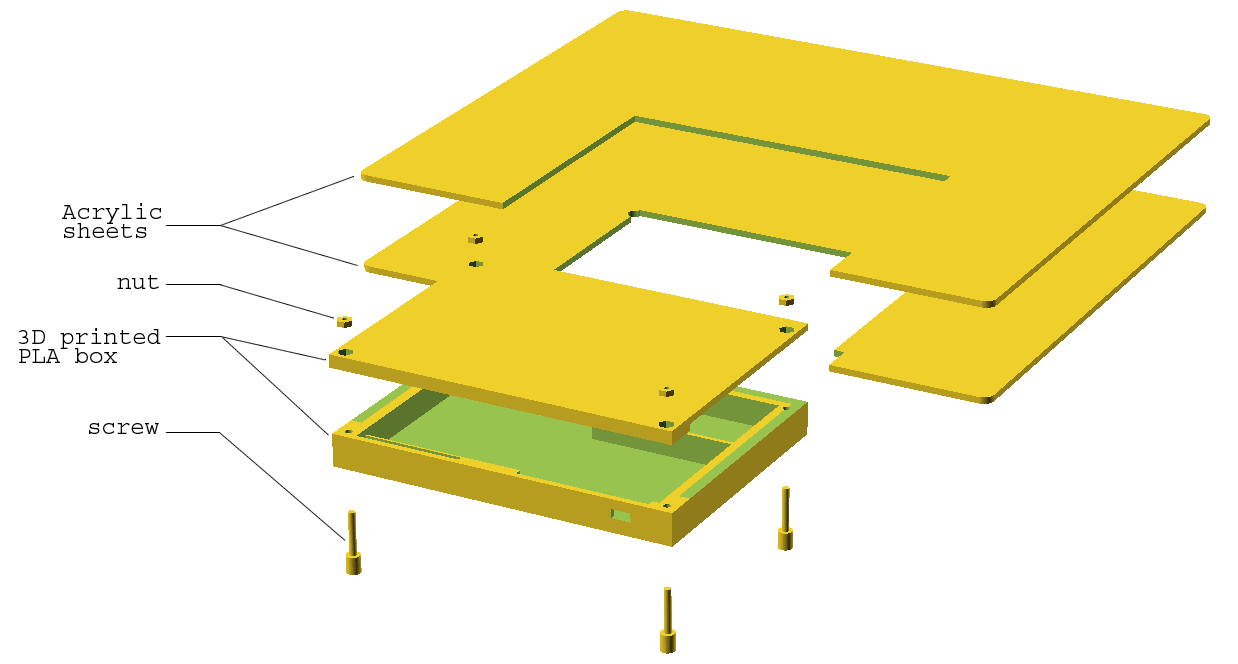
\includegraphics[width=1.2\textwidth]{figures/explode.png}} %
  \caption{\small {\it {Exploded view of the prototype.}}} 
  \label{fig:explode}
\end{figure}

\begin{figure}[h]
  \begin{minipage}[b]{.5\textwidth}
    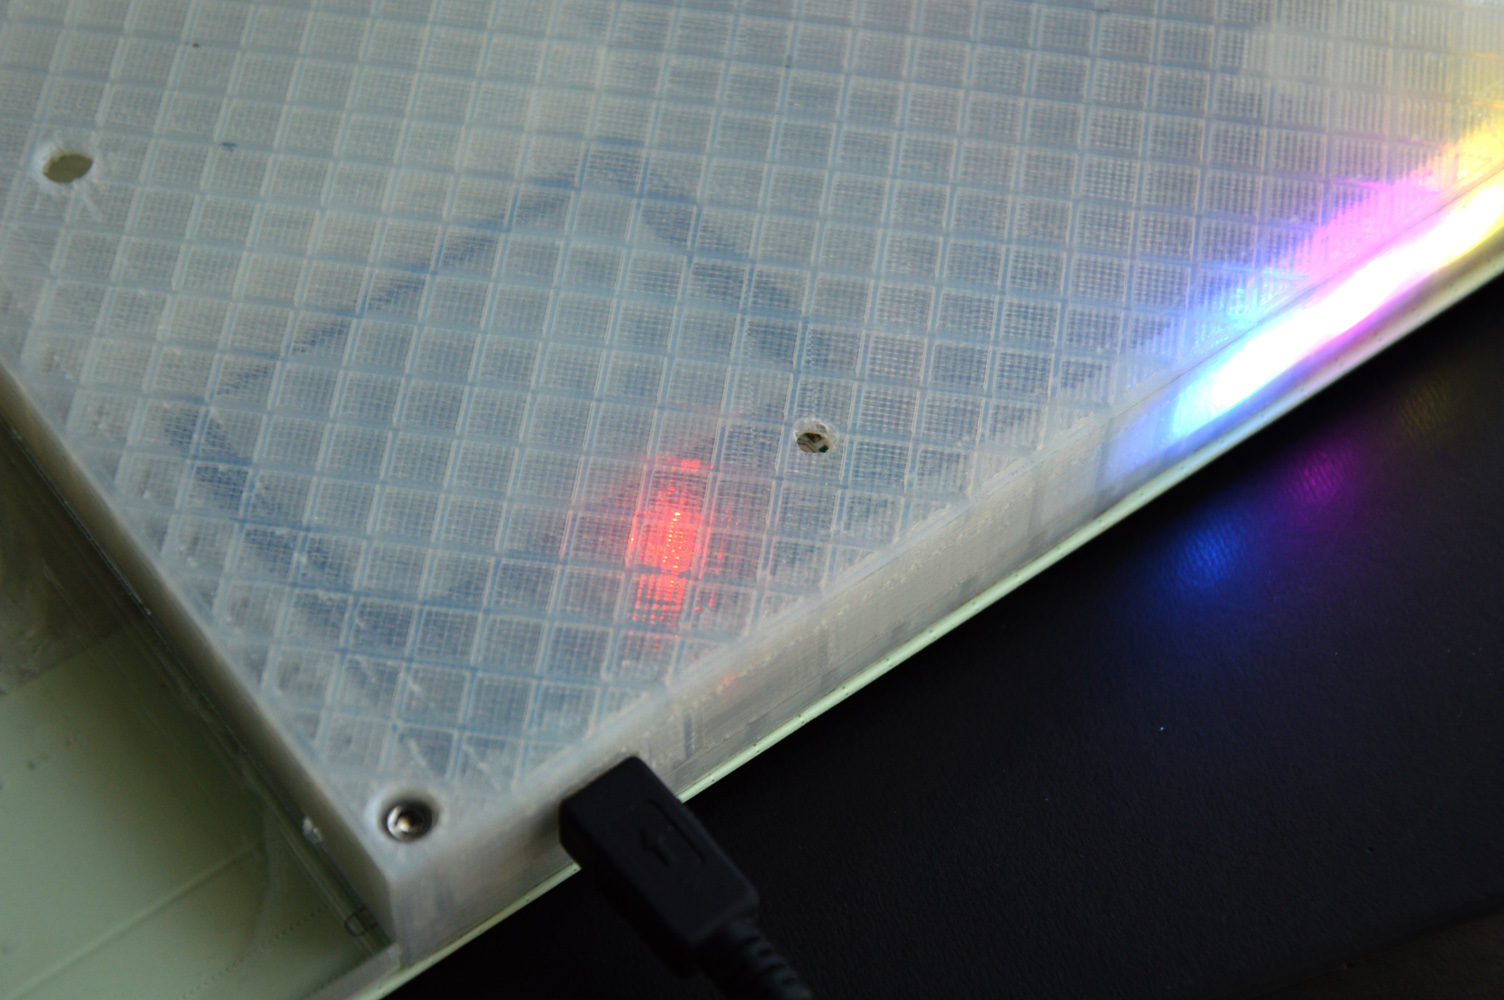
\includegraphics[width=1\textwidth]{figures/journal-charging.jpg}
  \end{minipage}
  \begin{minipage}[b]{.5\textwidth}
    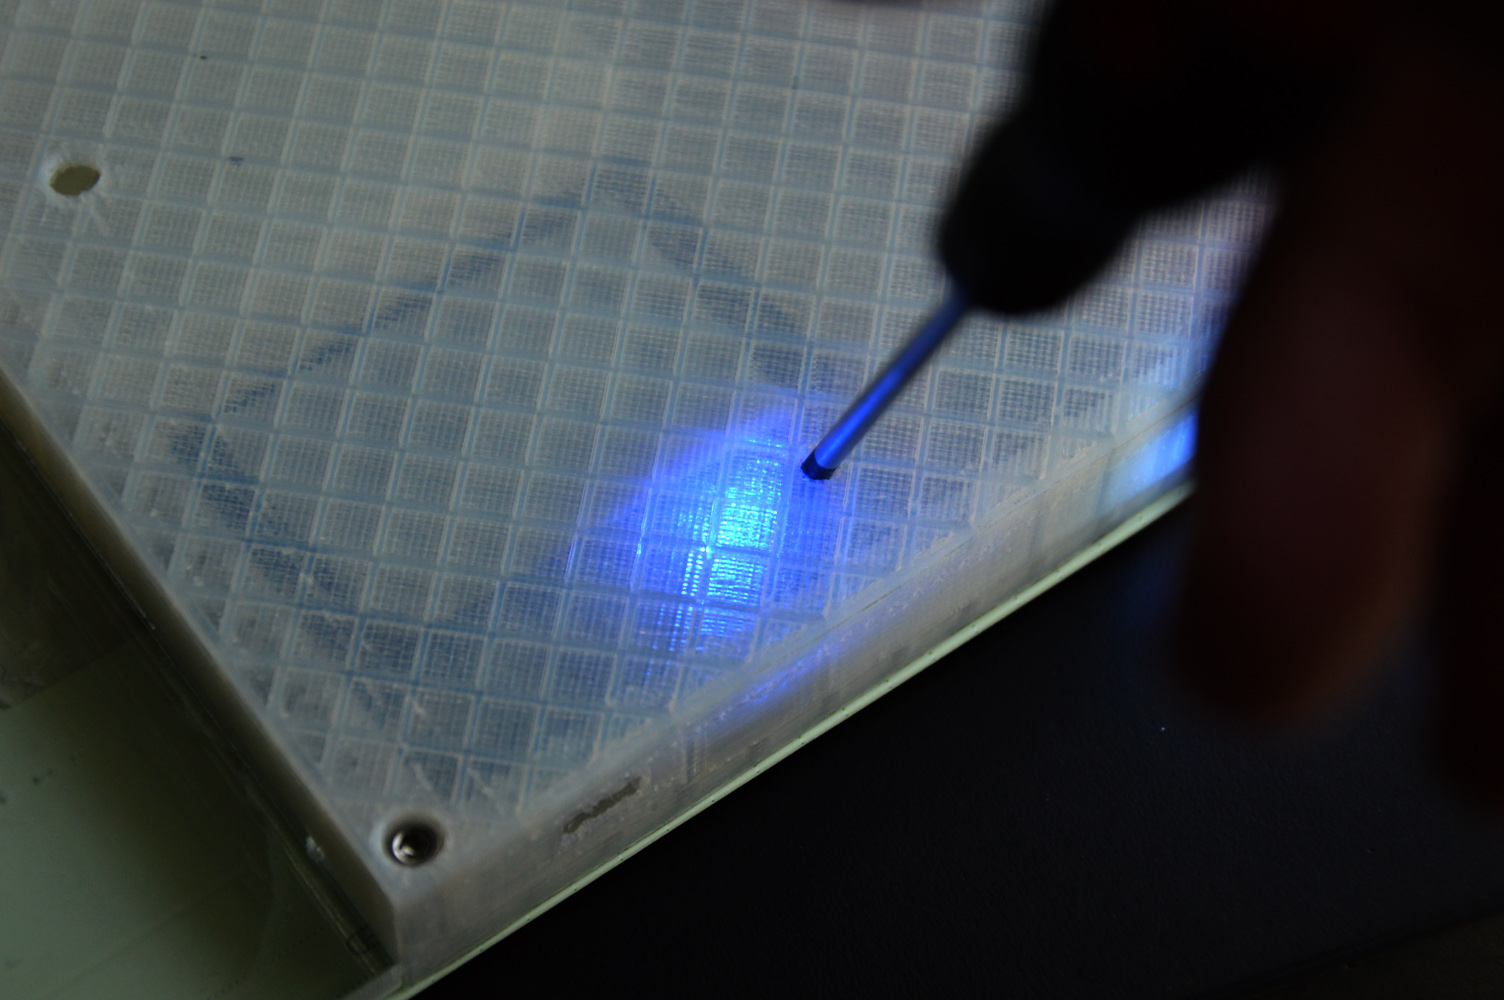
\includegraphics[width=1\textwidth]{figures/journal-battery.jpg}
  \end{minipage}
  \caption{\small {\it {Left: a red LED indicates charging state. Right: a button can be pressed to display battery status.}}} 
  \label{fig:journal-1}
\end{figure}


\begin{figure}[h]
  \makebox[\textwidth][c]{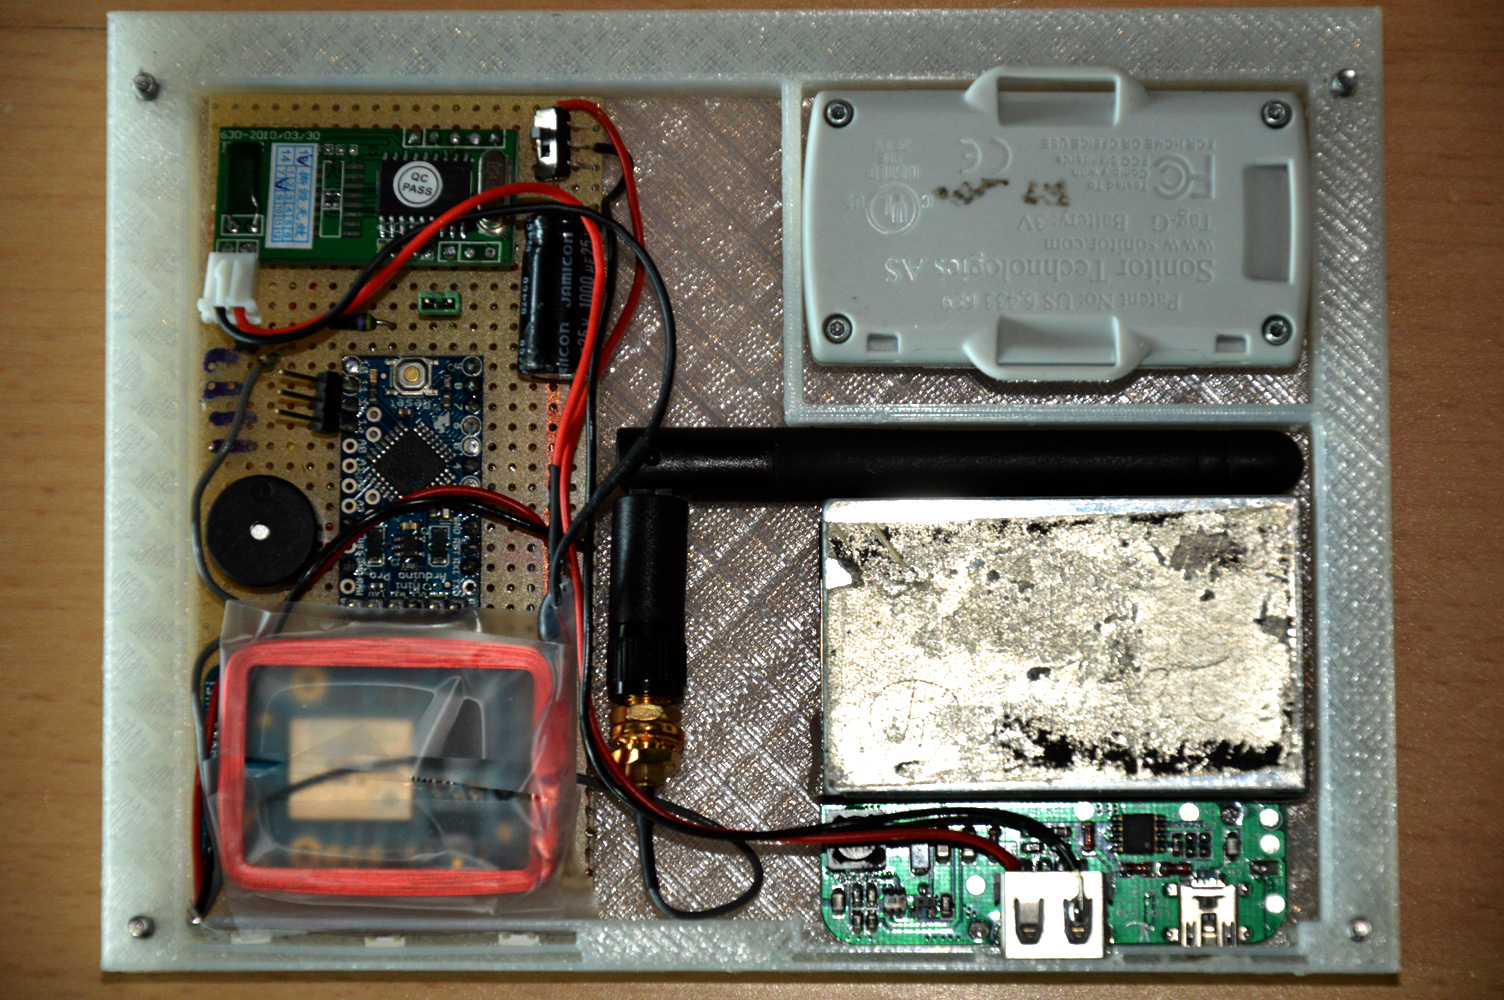
\includegraphics[width=1\textwidth]{figures/internals.jpg}}
  \caption{\small {\it {Inside the electronics compartment.}}} 
  \label{fig:internals}
\end{figure}


\clearpage

\section{Prototyping analysis}

Discussion of experience in building prototypes during the design process:
- Illustration of all the prototyping activities
- Discussion of specific areas where the experience of building prototypes affected the design requirements and specifications
% Discussion of experience in building prototypes during the design process:
% - Illustration of all the prototyping activities
% - Discussion of specific areas where the experience of building prototypes affected the design requirements and specifications



% Explanations of how to build the product, including information such as:
% - System architecture
% - Drawings and sketches
% - Parts and supply ordering information

% Design specifications marked for:
% - Quality
% - Accuracy
% - Originality

\subsection{Evaluation}
\subsubsection{Drop Test}
We did testing on the last iteration of our desgin, where we drop at a distance of 1 meter 10 times to simulate the fall from a desk, efter each time we locked for signs that ist was about to crack of fracture.
After the 10'th drop we started to see cracks in the acrylic, the cracks apired in the cutout section where there is a sharp courner, however this was only on the front acrylic plade, had we done the drop many more times we prolery whould have seen the same result in the back plate. 
This is properly due to the laser cutting, and could be avoid by making a round cut rathere that a sharp cut, or by drilling a hule to relive tension there might have been build up, during the laser cuting.

We did not check the hardware during the drop test, afterwards we tested the eletronic and found that it hadn't suffered any damage.

\subsubsection{Power Test}
For the power test we borrowed a discharger, from vaidas, where you can set the amount of amps it has to drain.
We calculated that the devise whould drain around 350 milliamps, if it runs at maximum capacity.
From that we found out that it would rund for 4 hours in the worst case, we later found out that if it is in idle mode, it can run for around 20 hours.

\subsubsection{Price}
Since we had to keep it under 1000 kr pr device, we locked around on the internet, to finde the cheapest parts.
the price for the acrylic is taken from RIAS where one 3mm thick $1 m^2$ acrylic is 532.
\begin{itemize} \itemsep0em
	 \item WIFI: 191 
	 \item Arduino: 54
	 \item RFID: 112,00 kr
	 \item Batterie: Free
	 \item LED: 7 kr
	 \item Charger: Free
	 \item Stepup converter: Free
	  \item Acryl: $(acrylic hight * acrylic width)*2 = 0,2 m^2 = 106.4 kr.$
	 \item Total: 470,4
\end{itemize}
If we had bought the stepup, charger and batteri we still would have been under the budgit limit.


\section{TESTING - ignore}

\begin{figure}[h]
\begin{center}
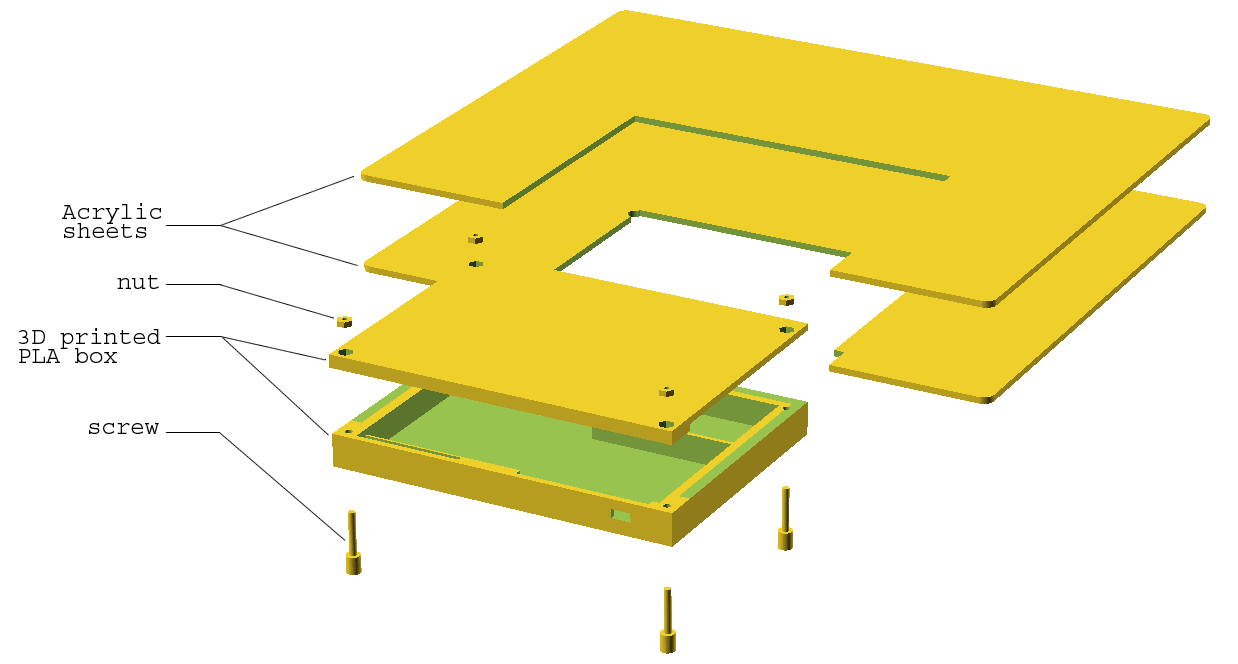
\includegraphics[scale=0.5]{figures/explode.png}
\caption{\small {\it {This is a description}}} \label{fig:explode}
\end{center}
\end{figure}


\begin{figure}[h]
\begin{minipage}[b]{7.5cm}
\centering
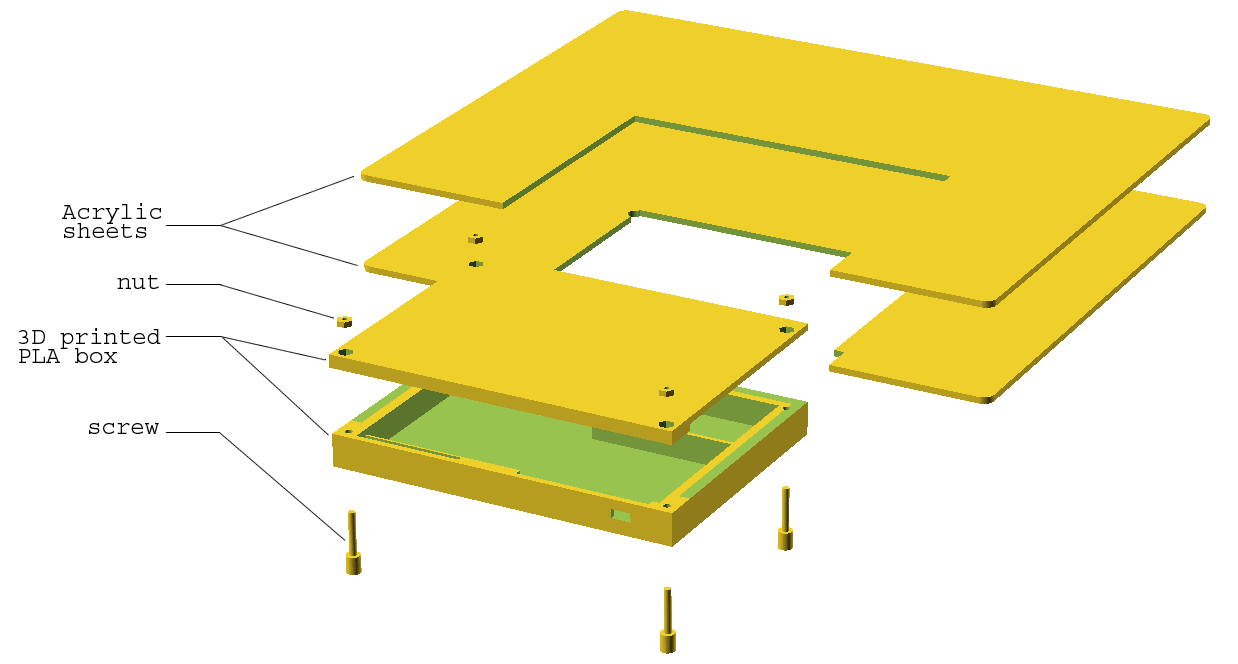
\includegraphics[scale=0.20]{figures/explode.png}
\caption{\small {\it {This is a description}}} \label{fig:testfig1}
\end{minipage}
\hspace{0.5cm}
\begin{minipage}[b]{7.5cm}
\centering
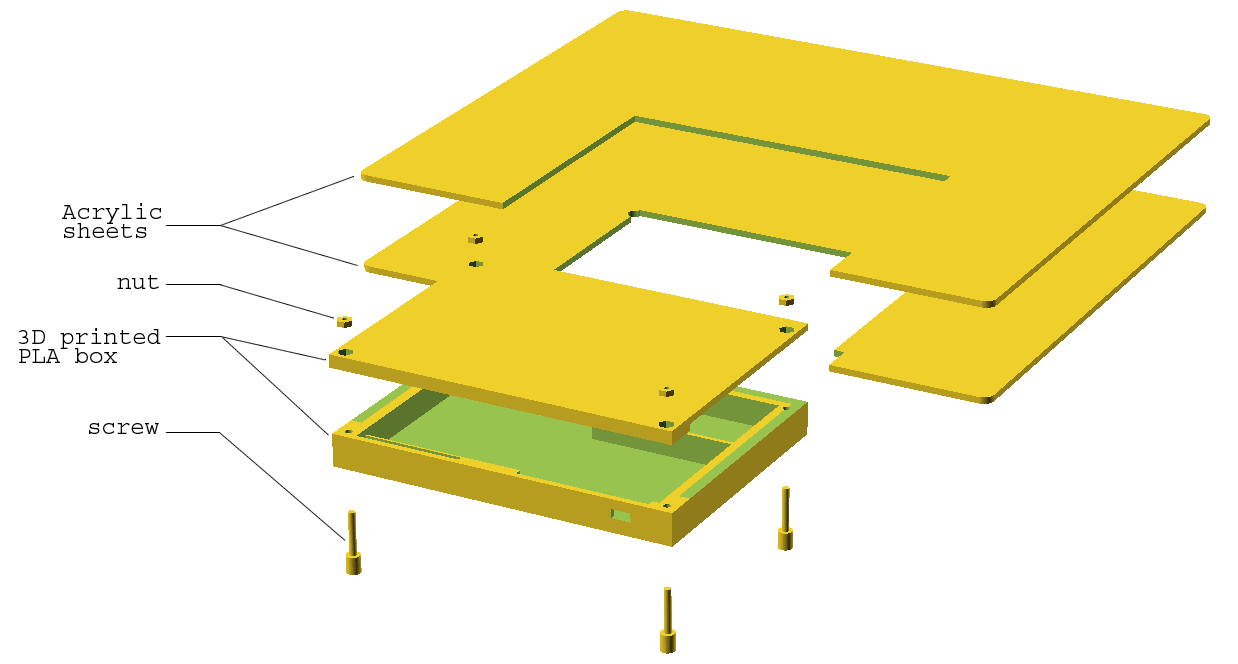
\includegraphics[scale=0.20]{figures/explode.png}
\caption{\small {\it {This is a description}}} \label{fig:testfig2}
\end{minipage}
\end{figure}


\begin{itemize} \itemsep0em
  \item The individual entries are indicated with a black dot, a so-called bullet \cite{chua2010}.
  \item The text in the entries may be of any length.
\end{itemize}


\section{Conclusions}


\clearpage

\bibliographystyle{plain}
\bibliography{References}



% \section{Electronic}

\title{Electronic}



% \section{Design}
\subsection{Materials}
We got a bunch of different plast materials from RIAS, in order to find some material that might be cheaper, and better that acrylic, since acrylic have tendency to be brittle, and this becomes worse when it has been laser cut. 

\subsection{Iterations}
we have used prototyping in order to get a viable device, through the different designs we have been able to see different problems, which have ment that we had to iterate to a new version, we have been limited by time, so we have had to make some compromises

\subsubsection{fisrt}
The first iteration that we build did have some problems.
The first is that it is expensive to build, since we are using a lot of acrylic, the secound point is that it still is heavy, and unwieldy.
But i did give some ideas for the next iteration.

\subsubsection{secound}


\subsubsection{thried}


\subsubsection{fourth}


\subsubsection{fith}



% \section{Problems}









\end{document}


%-----------------------------------------------
% Resources

http://www.me.umn.edu/education/undergraduate/writing/How-to-write-a-Design-Report.pdf

http://pastebin.com/raw.php?i=xudGnU7U

http://ocw.mit.edu/courses/sloan-school-of-management/15-783j-product-design-and-development-spring-2006/index.htm

